\chapter[Proposta]{Proposta}
Este capítulo apresenta detalhes sobre o \textit{framework} proposto neste trabalho de conclusão de curso. O capítulo está organizado em seções. Na seção 4.1, é explanado sobre os requisitos gerais do \textit{framework}. Em seguida, na seção 4.2, é apresentado os objetivos da prova de conceito. Na seção 4.3, é relatado os resultados obtidos até o momento.

\section{Framework para Geração de Teste Unitário} \label{ch4sec1}

A proposta deste trabalho é a implementação de um \textit{framework} capaz de dar suporte ao desenvolvedor na tarefa de produzir testes unitários.  Esse suporte deve ser capaz de gerar testes de forma semiautomatizada, visto que o programador deverá incluir no código especificações que guiem o \textit{framework} na criação dos testes unitários. 
\par
\indent A princípio, o \textit{framework} será desenvolvido com o intuito de gerar testes unitários em aplicações escritas em \textit{Grails}, especificamente para as operações básicas conhecidas como CRUD (\textit{create}, \textit{read}, \textit{update} e \textit{detele}). Entretanto, há intenção de evoluir o \textit{framework} para que ele seja compatível com demais métodos, bem como, com outras linguagens de programação. 
\par
\indent Para a implementação do \textit{framework}, será utilizada a linguagem de programação C++, junto com as ferramentas Flexc++ \cite{flexcpp2015} e Bisonc++ \cite{bisoncpp2015}. Essas ferramentas serão responsáveis pela análise léxica do código e \textit{parser} para geração da gramática, respectivamente. A ilustração a seguir fornece uma visão geral da arquitetura do \textit{framework} a  ser construído.
 
 \begin{figure}[h]
    \centering
    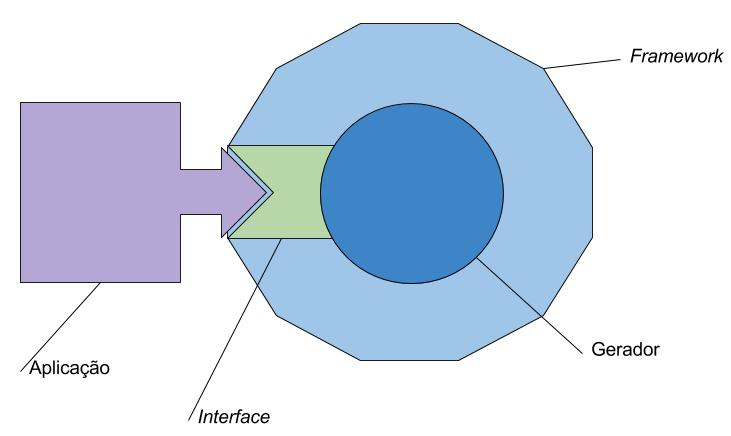
\includegraphics[width=0.7\textwidth]{figuras/estruturaarquitetural.jpg}
    \caption{Visão Geral do \textit{Framework}}
    \label{fig:estruturaarquitetural}
 \end{figure}

 \par
 \indent O \textit{framework} proposto possuirá em seu núcleo um gerador de testes unitários e, em uma camada mais elevada, possuirá uma interface com a função de possibilitar a interação com a aplicação. 
 
   \begin{figure}[h]
    \centering
    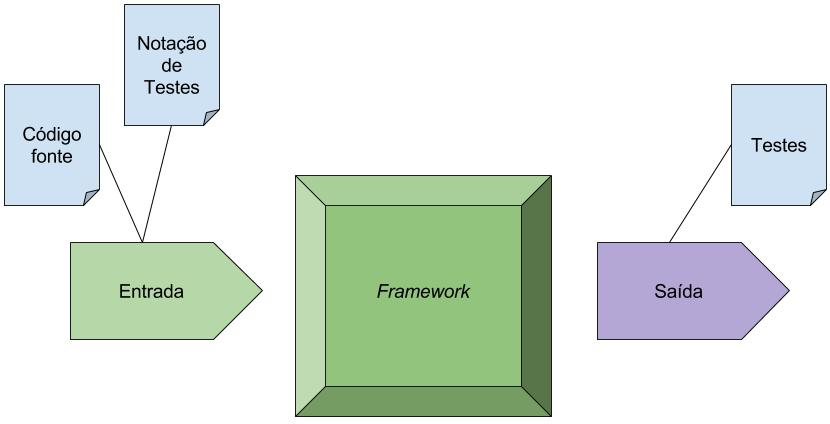
\includegraphics[width=0.7\textwidth]{figuras/entradasesaidas.jpg}
    \caption{Fluxo do funcionamento do \textit{Framework}}
    \label{fig:entradasesaidas}
 \end{figure}
 
 \par
\indent A Figura \ref{fig:entradasesaidas} enfatiza o fluxo do funcionamento do \textit{framework}. A entrada do \textit{framework} será o código fonte, bem como as especificações dos testes seguindo uma notação pré-determinada. Como saída, serão gerados os testes unitários conforme especifícados. O fluxo do funcionamento do \textit{framework} pode ser entendido, de forma simplificada, em quatro etapas: análise léxica, análise sintática, análise semântica e geração dos testes. 
 \begin{description}
 \item[Análise léxica:] onde será realizada a análise do código fonte de forma a reconhecer as palavras específicas, os \textit{tokens}. Essas palavras serão previamente definidas por meio do Flexc++ que fornece suporte para essa etapa \cite{flexcpp2015}.
 \item[Análise sintática:] ocorrerá uma avaliação do código fonte considerando as regras sintáticas definidas. Essas regras são formadas utilizando sequências de \textit{tokens}. Essa etapa será implementada com o auxílio do Bisonc++ cite{bisoncpp2015}.
 \item[Análise semântica:] será realizada uma interpretação do código apresentado verificando sua semântica, ou seja, será averiguado o significado dos \textit{tokens} identificados dentro do contexto.
  \item[Geração dos testes:] após as análises do código, será efetuado o \textit{parser} com o intuito de gerar os testes unitários específicados pelo desenvolvedor. Esses testes serão armazenados nos arquivos apropriados e serão a principal saída do \textit{framework}.
 \end{description}
 
 \begin{figure}[h]
    \centering
    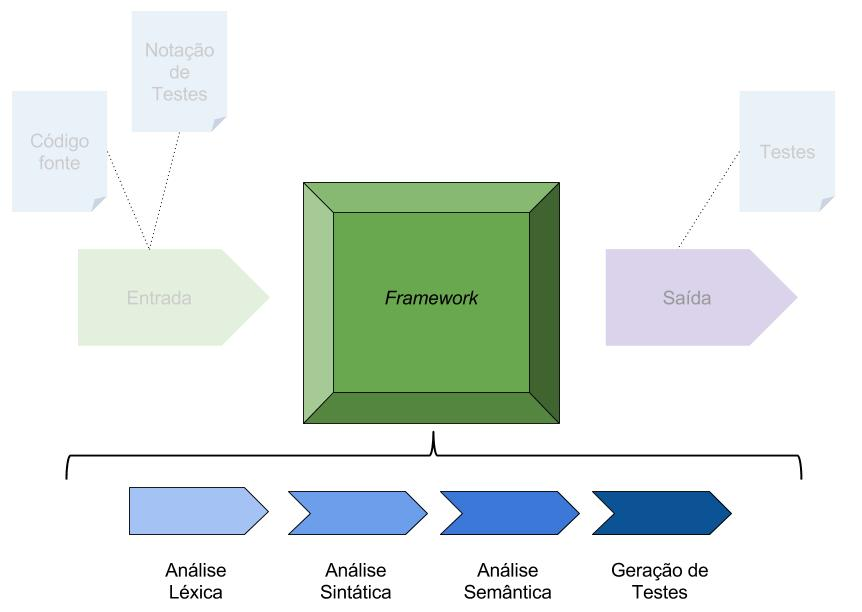
\includegraphics[width=0.9\textwidth]{figuras/Framework-interior.jpg}
    \caption{Fluxo do Funcionamento do \textit{Framework}}
    \label{fig:Framework-interior}
 \end{figure}
 
 \par
 \indent A Figura \ref{fig:Framework-interior} permite a visualização do fluxo básico do funcionamento do \textit{framework}.  


\subsection{Arquitetura do \textit{Framework}}



\subsection{Alvo Inicial: \textit{Grails}} 
\textit{Grails}, antigamente conhecido como \textit{Groovy on Grails}, é um \textit{web framework} para plataforma Java. Com o objetivo de propiciar maior produtividade ao desenvolvedor, \textit{Grail} faz uso do paradigma \textit{Convention-over-Configuration}.  Por ser integrado com a JVM (\textit{Java Virtual Machine}), \textit{Grails} possui diversas características, entre elas: a integração com ORM (\textit{Object Relational Mapping}), uso de uma \textit{domain-specific-language} e programação assíncrona \cite{grails2015}.
\par
\indent Devido ao fato de ser um \textit{web framework}, \textit{Grails} faz uso do padrão MVC (\textit{Model-View-Controller}), ou seja, as aplicações em \textit{Grails} separam a interação com usuário da representação da informação \cite{grails2015}.
\par
\indent \textit{Grails} utiliza-se de um sistema de comandos capaz de fornecer ao desenvolvedor a possibilidade de gerar código. Isso evita tarefas monótonas, mas necessárias, como funções básicas de \textit{models} e de \textit{controllers}. Esses métodos gerados podem ser modificados pelo desenvolvedor, conforme a necessidade de adequação ao contexto de trabalho  \cite{grails2015}.
\par
\indent Os geradores de código do \textit{Grails} produzem  \textit{stubs} para os testes. \textit{Stubs} são métodos ou classes vazias, contendo apenas cabeçalhos. Ao analisas os \textit{stubs} gerados, observa-se que eles são classes filhas do \textit{GroovyTestCase} que, por sua vez, é um \textit{facade} sobre o JUnit \cite{broughton2010}. Devido a isso, qualquer desenvolvedor que esteja familiarizado com o uso de funcionalidades comuns ao JUnit, como \textit{asserts}, \textit{setup} e \textit{teardown}, está apto a entender os testes em \textit{Grails} \cite{broughton2010}.
\par
\indent Abaixo segue um exemplo de um teste escrito utilizando o \textit{web framework Grails}:

\begin{lstlisting}[language=java, label=exTesteGrails, caption={Exemplo de Teste em \textit{Grails}}]
// Model
class HotelStay{
  String hotel
}

// Test
class HotelStayTests extends GroovyTestCase {
  void testSomething(){
    HotelStay hs = new HotelStay(hotel:"Sheraton")
    assertEquals "Sheraton", hs.hotel
  }
}
\end{lstlisting}

\subsection{Especificação dos Casos de Testes}
Como referenciado na seção \ref{ch4sec1}, será utilizado uma notação no código fonte que possibilitará ao desenvolvedor especificar seus casos de teste. Essa notação será inserida em comentários de documentação, permitindo assim, a especificação dos testes e a documentação dos mesmos, tudo centrado no código fonte.
\par
\indent Em essência, o desenvolvedor deverá ser responsável por definir quais serão as entradas dos testes e a saída esperada. Fazendo isso, o \textit{framework} será capaz de identificar esses valores e gerar os testes solicitados.

\section{Prova de Conceito}

\subsection{Bisonc++}

\subsection{Flexc++}

\subsection{Gerador de Teste Unitário}

\section{Resultados Obtidos}
 
\section{Resumo do Capítulo}
%%  Resumo do capítulo

 